\documentclass{article}
\usepackage[margin=0.6in]{geometry}
\usepackage{tikz}
\usetikzlibrary{positioning, shapes.callouts, arrows.meta}
\usepackage{booktabs}
\usepackage[table]{xcolor}
\usepackage{tcolorbox}
\usepackage{array}
\usepackage{adjustbox}
\usepackage{amsmath}
\usetikzlibrary{fit, calc}
\tikzset{
  arrow/.style={-Latex, thick, line width=4.2pt, draw=gray!50},
}

\pagestyle{empty}

\begin{document}

% Question
Q: How many points per game did Lebron James get in the NBA Season suspended by COVID? \hfill A: 25.3
\begin{figure}[ht]
\centering
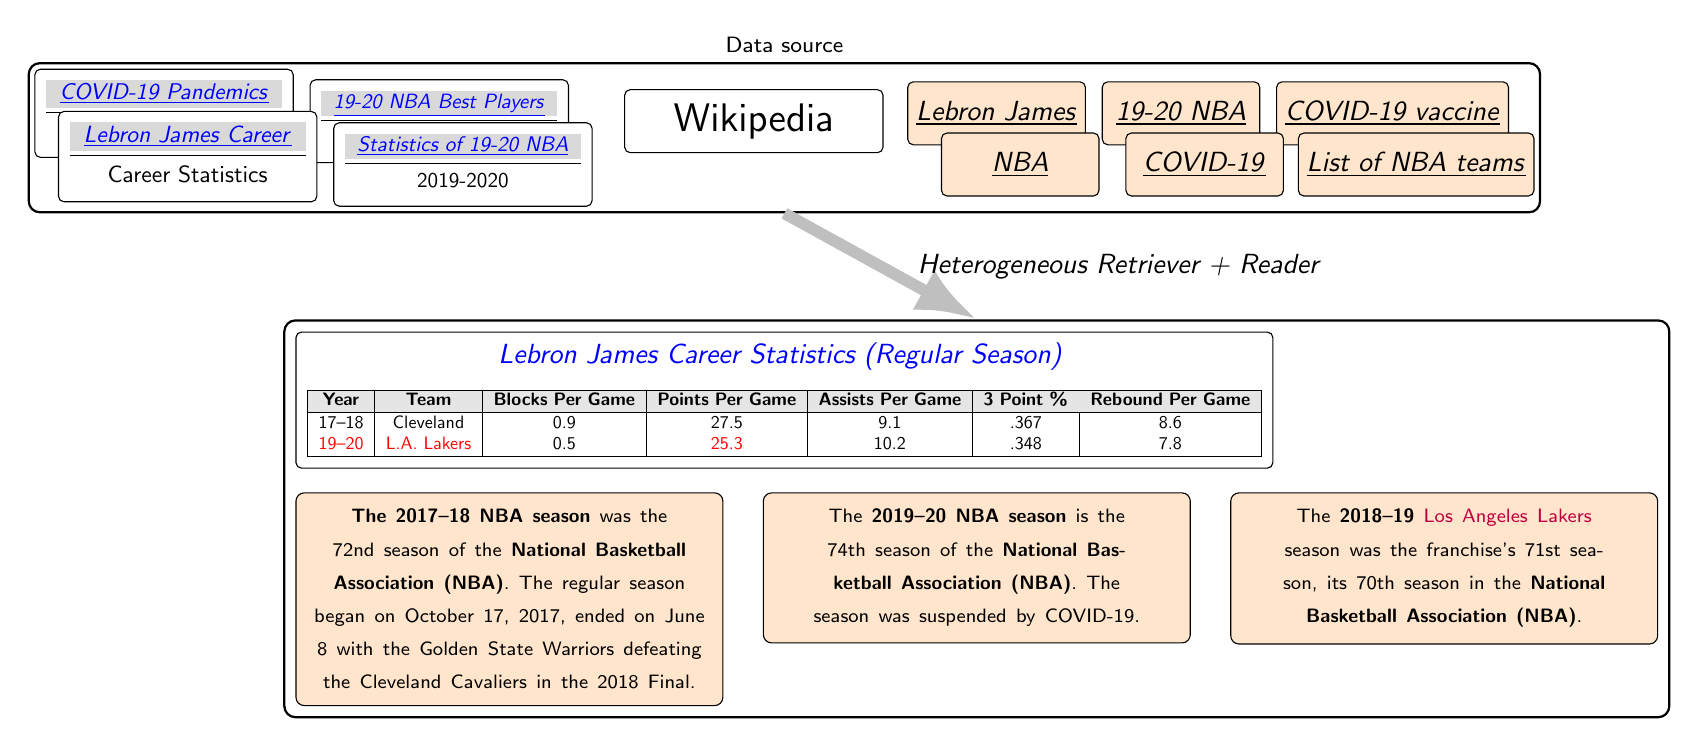
\begin{tikzpicture}[
  every node/.style={font=\sffamily},
  box/.style={draw, fill=white, text width=3cm, align=center, rounded corners=2pt, inner sep=4pt, minimum height=0.8cm},
  yellowbox/.style={draw, fill=orange!20, align=center, rounded corners=2pt, inner sep=3pt, minimum height=0.8cm, minimum width=2cm},
  tanbox/.style={draw, fill=orange!20, text width=5cm, align=center, inner sep=6pt, rounded corners=3pt},
  nobox/.style={draw=none, fill=none, align=center, inner sep=0pt},
  node distance=0.4cm and 0.2cm
]

% Top-level source tiles (row 1)
\node[box] (covid) {
\begin{adjustbox}{max width=\textwidth}
  \begin{tabular}{c}
  \rowcolor{gray!30}
  {\color{blue}\underline{\textit{COVID-19 Pandemics}}} \\ \midrule 
  Report
  \end{tabular}
  \end{adjustbox}
  };
  
\node[box, right= of covid, yshift=-0.1cm] (players1920) {
\begin{adjustbox}{max width=\textwidth}
  \begin{tabular}{c}
  \rowcolor{gray!30}
  {\color{blue}\underline{\textit{19-20 NBA Best Players}}} \\ \midrule 
  List of MVPs
  \end{tabular}
  \end{adjustbox}
  };
  
\node[box, xshift=0.3cm] at ([yshift=-0.55cm]covid) (stats) {
\begin{adjustbox}{max width=\textwidth}
  \begin{tabular}{c}
  \rowcolor{gray!30}
  {\color{blue}\underline{\textit{Lebron James Career}}} \\ \midrule 
  Career Statistics
  \end{tabular}
  \end{adjustbox}
  };

\node[box, xshift=0.3cm] at ([yshift=-0.55cm]players1920) (stats1920) {
\begin{adjustbox}{max width=\textwidth}
  \begin{tabular}{c}
  \rowcolor{gray!30}
  {\color{blue}\underline{\textit{Statistics of 19-20 NBA}}} \\ \midrule 
  2019-2020
  \end{tabular}
  \end{adjustbox}
  };

%Middle box written Wikipedia    
\node[box, right= 0.7cm of players1920] (wiki) {\Large Wikipedia};

% Right-side tiles
\node[yellowbox, right= 0.3cm of wiki, yshift=0.1cm] (lebron) {\underline{\textit{Lebron James}}};
\node[yellowbox, right= of lebron] (nba1920) {\underline{\textit{19-20 NBA}}};
\node[yellowbox, right= of nba1920] (vaccine) {\underline{\textit{COVID-19 vaccine}}};
\node[yellowbox, xshift=0.3cm] at ([yshift=-0.65cm]lebron) (nba) {\underline{\textit{NBA}}};
\node[yellowbox, xshift=0.3cm] at ([yshift=-0.65cm]nba1920) (covid19) {\underline{\textit{COVID-19}}};
\node[yellowbox, xshift=0.3cm] at ([yshift=-0.65cm]vaccine) (teams) {\underline{\textit{List of NBA teams}}};

% Surrounding box for data source
\node[draw, thick, rounded corners, inner sep=2pt, fit=(covid) (players1920) (stats) (stats1920) (lebron) (nba1920) (vaccine) (nba) (covid19) (teams), label=above:{\footnotesize Data source}] (datasource){};
  
% Table 
\node[draw, text width=\textwidth, align=center, below= 1.5cm of datasource, rounded corners=2pt, inner sep=4pt] (table){
\parbox{\linewidth}{\centering
\textit{\textcolor{blue}{Lebron James Career Statistics (Regular Season)}} \vspace{0.6em}}

\begin{adjustbox}{max width=\textwidth}
\begin{tabular}{|c|c|c|c|c|c|c|}
\hline
\rowcolor{gray!20}
\textbf{Year} & \textbf{Team} & \textbf{Blocks Per Game} & \textbf{Points Per Game} & \textbf{Assists Per Game} & \textbf{3 Point \%} & \textbf{Rebound Per Game} \\
\hline
17--18 & Cleveland & 0.9 & 27.5 & 9.1 & .367 & 8.6 \\
\textcolor{red}{19--20} & \textcolor{red}{L.A. Lakers} & 0.5 & \textcolor{red}{25.3} & 10.2 & .348 & 7.8 \\
\hline
\end{tabular}
\end{adjustbox}
};

% Bottom callout boxes
\node[tanbox, below left = 0.3cm and 0cm of table, anchor=north west] (explain1) {
\scriptsize\textbf{The 2017--18 NBA season} was the 72nd season of the \textbf{National Basketball Association (NBA)}. The regular season began on October 17, 2017, ended on June 8 with the Golden State Warriors defeating the Cleveland Cavaliers in the 2018 Final.
};

\node[tanbox, anchor=north west] at ([xshift=0.5cm]explain1.north east) (explain2) {
\scriptsize The \textbf{2019--20 NBA season} is the 74th season of the \textbf{National Basketball Association (NBA)}. The season was suspended by COVID-19.
};

\node[tanbox, anchor=north west] at ([xshift=0.5cm]explain2.north east) (explain3) {
\scriptsize The \textbf{2018--19} \textcolor{purple}{Los Angeles Lakers} season was the franchise's 71st season, its 70th season in the \textbf{National Basketball Association (NBA)}.
};

% Surrounding box for knowledge retrieval
\node[draw, thick, rounded corners, inner sep=4pt, fit=(table) (explain1) (explain2) (explain3)] (retrieval){};

% Arrow down 
\draw[arrow] (datasource.south) -- node[nobox, right, xshift=0.4cm] {\textit{Heterogeneous Retriever + Reader}} (retrieval.north);


\end{tikzpicture}
\caption{The problem setting: A OTT-QA model needs to retrieve from two candidate pools and then perform multi-hop reasoning to find answers.}
\end{figure}

\end{document}
